\chapter{Topologie řídícího systému dronu}

Práce se zaobírá v první řadě simulací bezpilotních letadel ve virtuálním prostředí, ale z důvodu možné budoucí realizace projektu je nutné pracovat s konkrétními hardwarovými a softwarovými řešeními.

Topologii řídícího systému dronu jsme rozdělili na dvě části. Palubní počítač řídí bezpilotní misi a řídící jednotka ovládá kritické procesy v dronu. Na trhu existuje nepřeberné množství různých komponentů pro autonomní mise. Na základě existujících projektů, například \textit{Multi Robot Systems Group} z ČVUT, \cite{MRS} jsme zvolili modul Pixhawk jako řídící jednotku. Jako palubní počítač, který ovládá samotnou autonomní misi jsme zvolili jednodeskový počítač Raspberry PI.

S touto kombinací jsme schopni řídit velké množství různých autonomních letadel a vozidel jako jsou:

\begin{itemize}
    \item dron v různých konfiguracích
    \item delta \acs{VTOL} (\acl{VTOL})
    \item letadlo v různých konfiguracích
    \item vrtulník
    \item rover
    \item ponorka
\end{itemize}

\section{Řídící jednotka Pixhawk}

Pixhawk je otevřený hardwarový projekt, jehož cílem je poskytnout standard\break pro snadno dostupné a vysoce kvalitní návrhy hardwaru autopilota pro akademické, vývojářské a hobby komunity. \cite{PIX1}

Řídící jednotka Pixhawk se využívá pro řízení kritických procesů v dronu jako jsou \textit{fail safe} funkce, ovládání pohonů, stabilizace a čtení kritických snímačů jako jsou GPS, barometr a \acs{IMU} (\acl{IMU}). Do jednotky Pixhawk je možné posílat řídící povely z RC vysílačky, a je možné do ní nahrát jednoduchou bezpilotní misi pomocí software QGroundControl nebo MissionPlanner.

Existuje několik variant řídící jednotky od značky Pixhawk:

\begin{itemize}
    \item Pixhawk (výroba byla ukončena)
    \item Pixhawk 2 (výroba byla ukončena)
    \item Pixhawk 3 Pro
    \item Pixhawk 4
    \item Pixhawk 4 Mini
    \item Pixhawk 5X
    \item Pixracer
    \item Auterion Skynode (průmyslové řešení)
\end{itemize}

Na obrázku \ref{fig:PIX} je zobrazena řídící jednotka Pixhawk 4. Můžeme si na ní všimnout redundantní porty pro napájení (\texttt{POWER1, POWER2, USB}), sběrnice \texttt{I2C, SPI, CANbus, UART, S.BUS}. Velkou výhodou je nízká hmotnost, která činí jenom 15,8g. \cite{PX4docs} %(\url{https://docs.px4.io/master/en/flight_controller/pixhawk4.html})

\begin{figure}[!ht]
    \begin{center}
        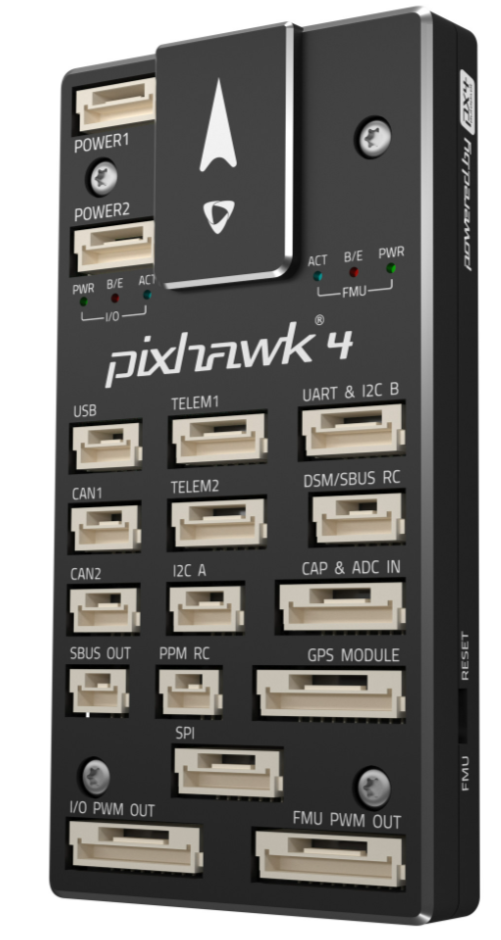
\includegraphics[scale=0.47]{obrazky/PIX}
    \end{center}
    \caption[Řídící jednotka Pixhawk 4]{Řídící jednotka Pixhawk 4 \cite{PX4docs}.}
    \label{fig:PIX}
\end{figure}

Mezi hlavní výhody řídících jednotek Pixhawk patří kvalitní softwarová podpora, automatické aktualizace firmware pomocí QGroundControl software, flexibilita\break z hlediska připojených hardwarových periferií a silná komunita uživatelů a vývojářů. Jednotka Pixhawk podporuje simulaci \acs{HITL} (\textit{\acl{HITL}}), což umožňuje test firmwaru a komunikace ještě před samotným vzletem dronu.

\section{Palubní počítač}

Jako palubní počítač se na experimentální letecké mise využívá jednodeskový počítač Raspberry PI. Na trhu existuje množství různých variant tohoto široce rozšířeného počítače v rozmezí od levného, malého a úsporného  \textit{Raspberry PI Pico}, až po vysoce výkonný počítač \textit{Raspberry PI 4B}.

Důležitými výhodami pro aplikace v robotických misích jsou integrace na jeden plošný spoj, nízká proudová spotřeba a možnost spuštění linuxových distribucí. Nejběžnější podporované distribuce jsou Raspberry PI OS, Raspbian, Ubuntu desktop a server.

Hlavní důvod pro použití Raspberry PI jako palubního počítače je možnost spolehlivé komunikace s firmware pro řízení bezpilotních letadel (PX4, ArduPilot, ...) přes ROS 2 \textit{topic}, nebo MAVLink. Komunikací mezi uvedenými platformami se budeme zabývat v následujících kapitolách.
